\htwo{Responsive Design}
\sectionauthor{Johannes Polzer}
\hthree{Allgemeines Projektmanagement}
\sectionauthor{Richard Panzer}

Projektmanagement ist wichtig, um ein Projekt zu strukturieren, zu planen und im Endeffekt zeitgerecht fertigzustellen. Ein Projekt im Allgemeinen ist ein Auftrag, welcher zeitlich begrenzt, risikobehaftet und daher auch von allen anderen Tagesgeschäften eines Unternehmens abgegrenzt ist. Da ein Projekt meistens recht komplex ist, ist die Rolle eines Projektmanagers eingeführt worden, um den gesamten Ablauf, welcher auch zwischen mehreren Abteilungen passieren kann, zu betreuen. \cite{Projectman.}

Im Laufe der Zeit entwickelten viele Leute unterschiedliche Ansätze im Projektmanagement, um ein Projekt abzuwickeln und es im Endeffekt als erfolgreich abgehakt werden kann. Diese unterschiedlichen Ansätze gibt es, da ein Projekt nicht gleich ein Projekt ist und eine klassischere Art (siehe Kapitel \ref{sec:klassisch}, Seite \pageref{sec:klassisch}) besser zu einem Projekt passt, während zu einem anderen Projekt die agilere Methode (siehe Kapitel \ref{sec:agile}, Seite \pageref{sec:agile}) bei der Abwicklung besser funktioniert. \cite{Projectman.}

In den folgenden Kapiteln wird sowohl auf klassisches als auch auf agiles Management eingegangen und das Management in \ZELIA\ wird beleuchtet. \cite{Projectman.}



\hthree{Anwendung}

Bei der Software \ZELIA\ erlauben zwei grundlegende Möglichkeiten das Ziel einer "responsive" Webseite, welche auf allen Geräten verwendet werden kann, zu erfüllen.

\begin{itemize}
    \item Media Queries -- vergleiche \ref{sec:mediaQueries}
    \item Clamp-Funktion -- vergleiche \ref{sec:clamp}
\end{itemize}

\hfour{Media Queries}\label{sec:mediaQueries}

"CSS-Media-Queries" ermöglichen es Webentwicklern, Styles für eine Webseite in Abhängigkeit von Medientyp, Ansichtsgröße und Ausrichtung zu schreiben. 
Die "View Size" ist die Größe des Inhalts, der auf einem Bildschirm gleichzeitig angezeigt werden kann, und wird in Pixeln gemessen. 
Es ist auch möglich, die Webseite anders zu gestalten, je nachdem, ob sie auf dem Bildschirm angezeigt oder ausgedruckt wird. 

\begin{minipage}{\textwidth}
    Jede Media Query hat folgende Struktur:
    
    \css{code/ResponsiveDesign/MediaQueries.css}{Beispiel Media-Queries}
\end{minipage}

Es gibt drei verschiedene Medien, auf die ein unterschiedliches Design angewandt werden kann: 
\begin{itemize}
    \item screen: Style wird nur auf dem Bildschirm angewandt.
    \item print: Style wird auf die Druckfunktion angewandt.
    \item speech: CSS wird nur von Plastischen Readern verwendet, welche den Text vorlesen.
\end{itemize}

Zusätzlich gibt es die Option "all", welche alle drei "media-types" beeinflusst. \cite{w3MediaQueries}

Beispiele für "media-features" sind

\begin{itemize}
    \item max-width: beeinflusst kleinere Bildschirme als die angegebene Größe
    \item min-width: beeinflusst größere Bildschirme als die angegebene Größe 
    \item orientation: prüft, ob das Gerät im horizontalen oder vertikalen Modus verwendet wird
    \item prefers-color-scheme: prüft, ob das Gerät ein helles oder dunkles Theme verwendet
\end{itemize}

\hfour{Clamp Funktion}\label{sec:clamp}

Die Clamp-Funktion ermöglicht es, ein Element dynamisch zu skalieren, ohne dafür Media-Queries zu verwenden. 
Dazu übernimmt sie drei Parameter. Der erste ist der Minimalwert. 
Dieser wird in einer fixen Einheit, wie \zb\ Pixel (px), angegeben. 
Der zweite Parameter gibt den optimalen Wert an. 
Dieser wird in einer Einheit angegeben, welche abhängig von der Breite des Bildschirms (vw) bzw. dem übergeordneten HTML-Element (\%) ist. 
Der dritte Parameter ist die Maximalbreite. 
Dieser funktioniert, so wie die Minimalbreite. 

Die Einheit {\ttfamily vw} steht für "Viewport Width" und gibt prozentuell die Breite relativ zum Viewport an. Der Viewport ist die Größe des Bereiches der Web-App, welcher am Bildschirm gleichzeitig angezeigt werden kann. 
Mit dem Prozentzeichen ("{\ttfamily \%}") kann die Größe relativ zum übergeordneten Element angegeben werden

Das folgende Element wird von mindestens 100 Pixel mit 80-prozentiger Bildschirmbreite bis zu 800px Breite skaliert.

\css{code/ResponsiveDesign/clamp.css}{Beispiel "clamp"-Funktion}

\clearpage
\hthree{Beispiele}
\hfour{Vergleich: Light- und Dark-Theme}

Die \ZELIA\ App lässt sich sowohl im Light- als auch im Dark-Theme anzeigen (siehe Abbildung \ref{fig:theme}). Dafür werden Media Queries (siehe Kapitel \ref{sec:mediaQueries}) verwendet, welche das Theme des Browsers abfragen (siehe Code \ref{code:theme}). 
Die jeweiligen Farben werden in CSS-Variablen gespeichert. Dadurch müssen die Farben nur einmal in einer Media Query angepasst werden und können nun für jedes Element verwendet werden. 

\begin{figure}[H]
    \begin{subfigure}[c]{0.49\textwidth}
        \centering
        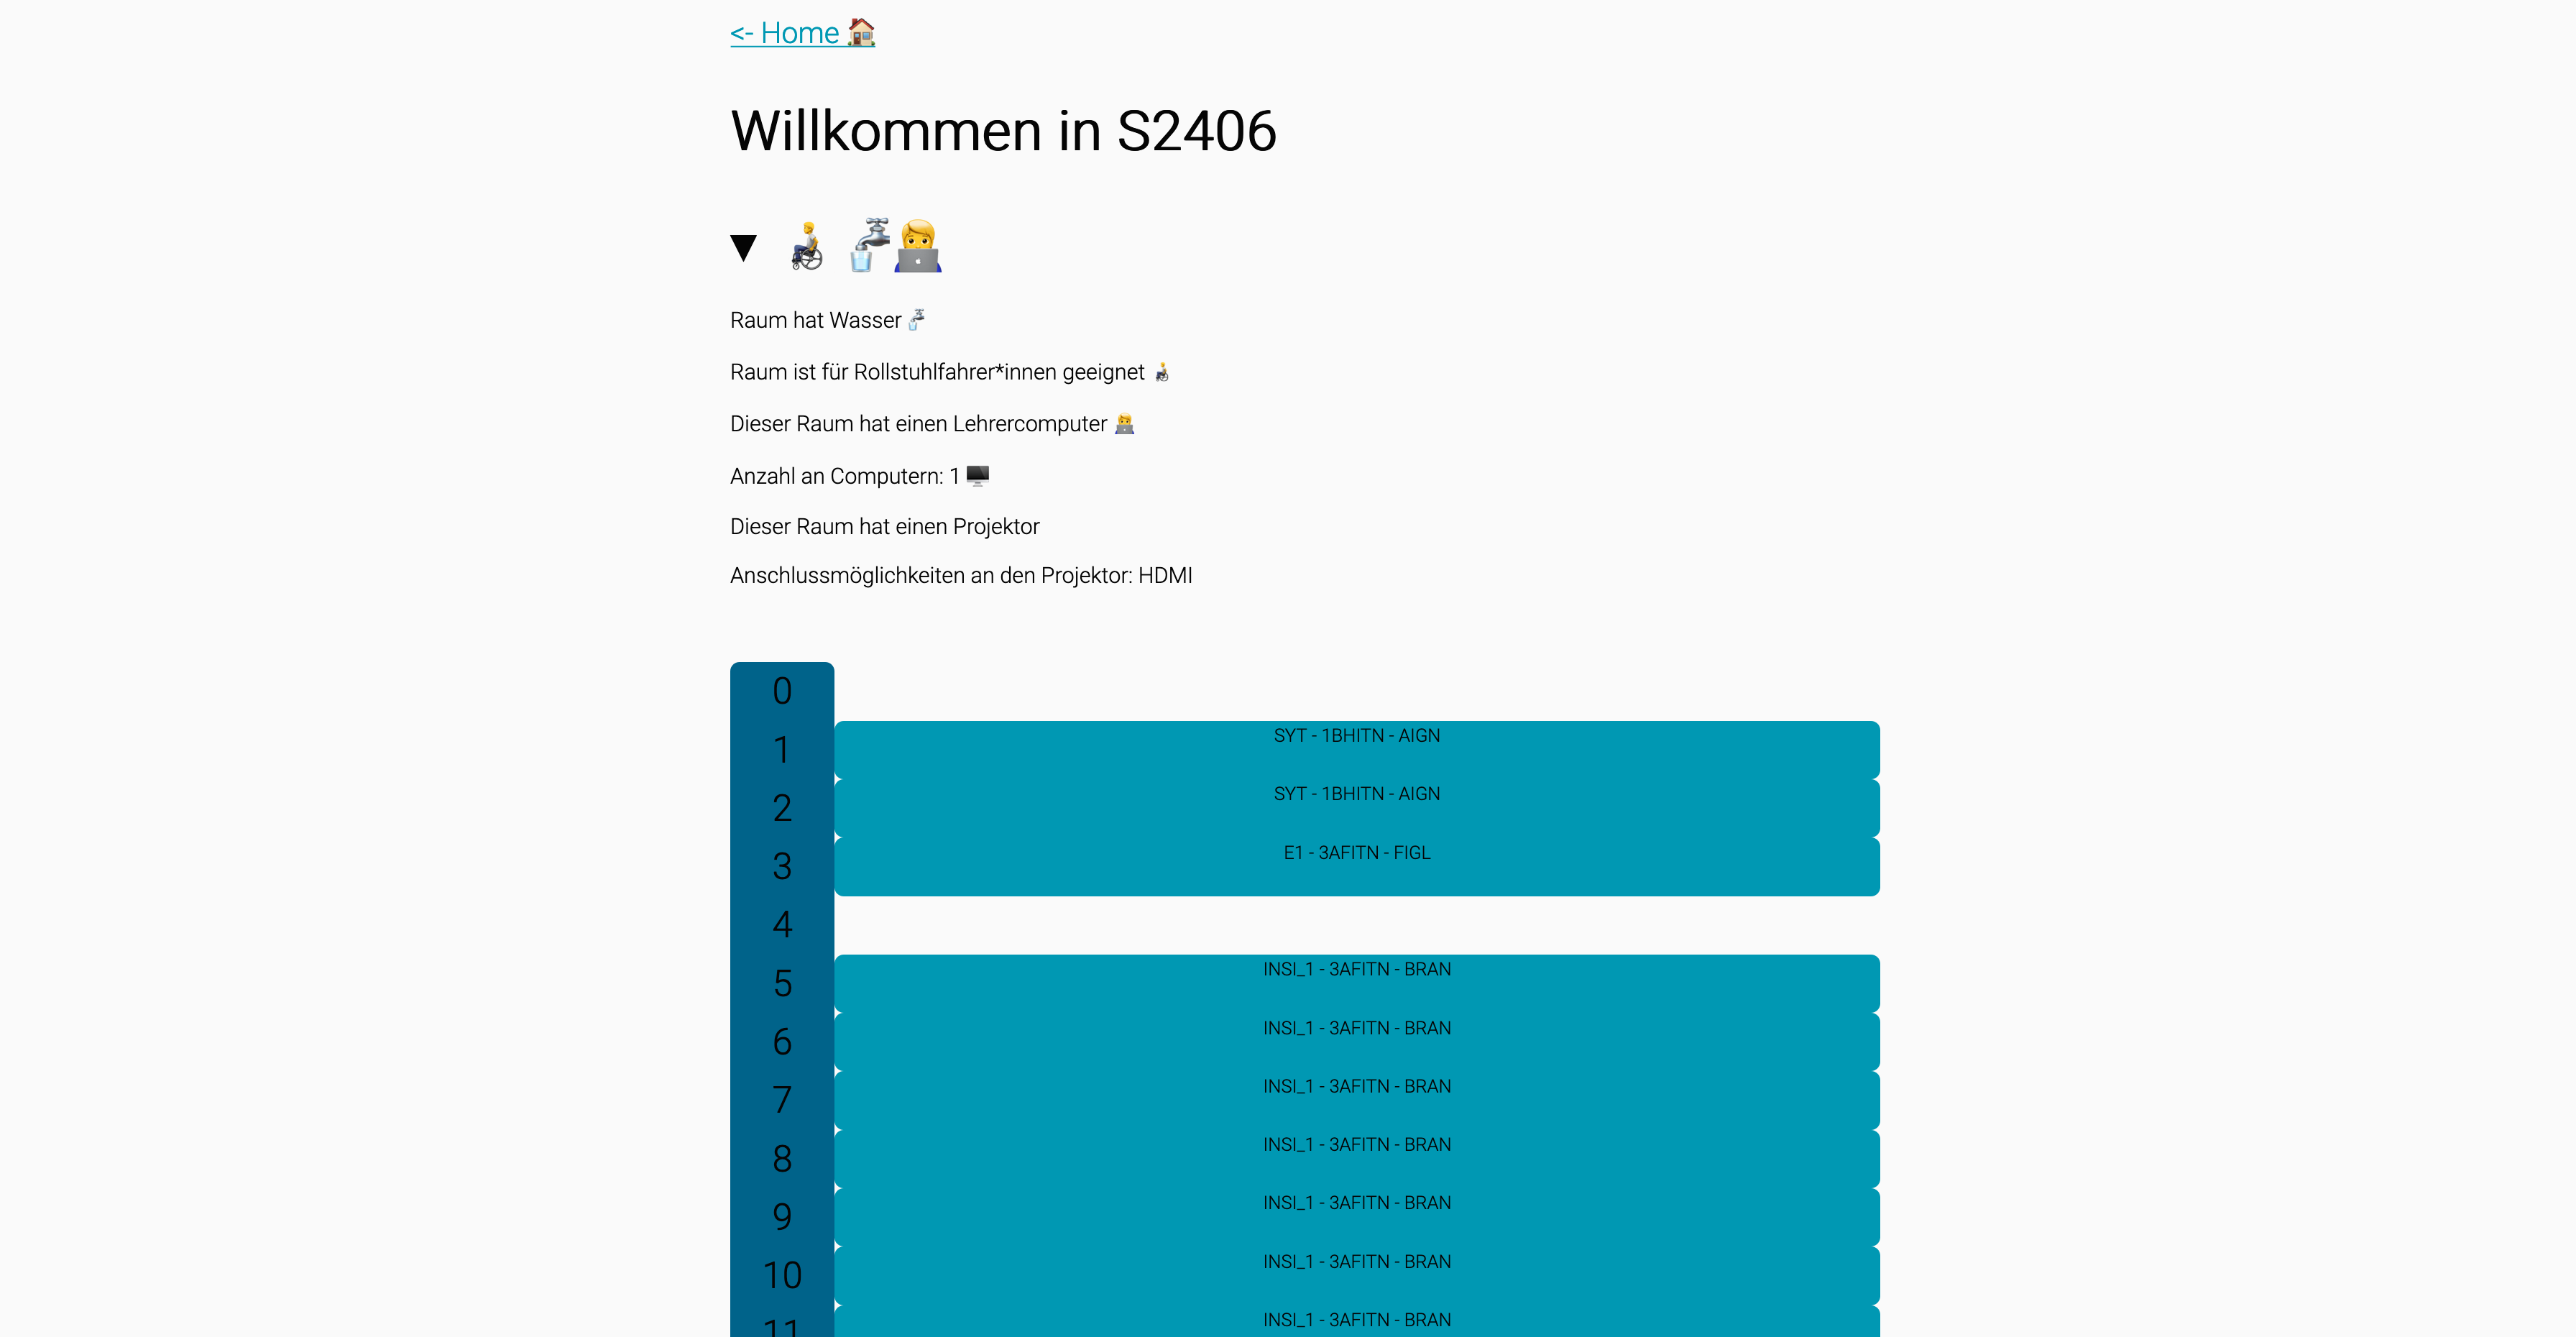
\includegraphics[width=\textwidth]{media/ResponsiveDesign/ZeliaDesktop.png}
        \caption{Helles Theme}
    \end{subfigure} \hfill
    \begin{subfigure}[c]{0.49\textwidth}
        \centering
        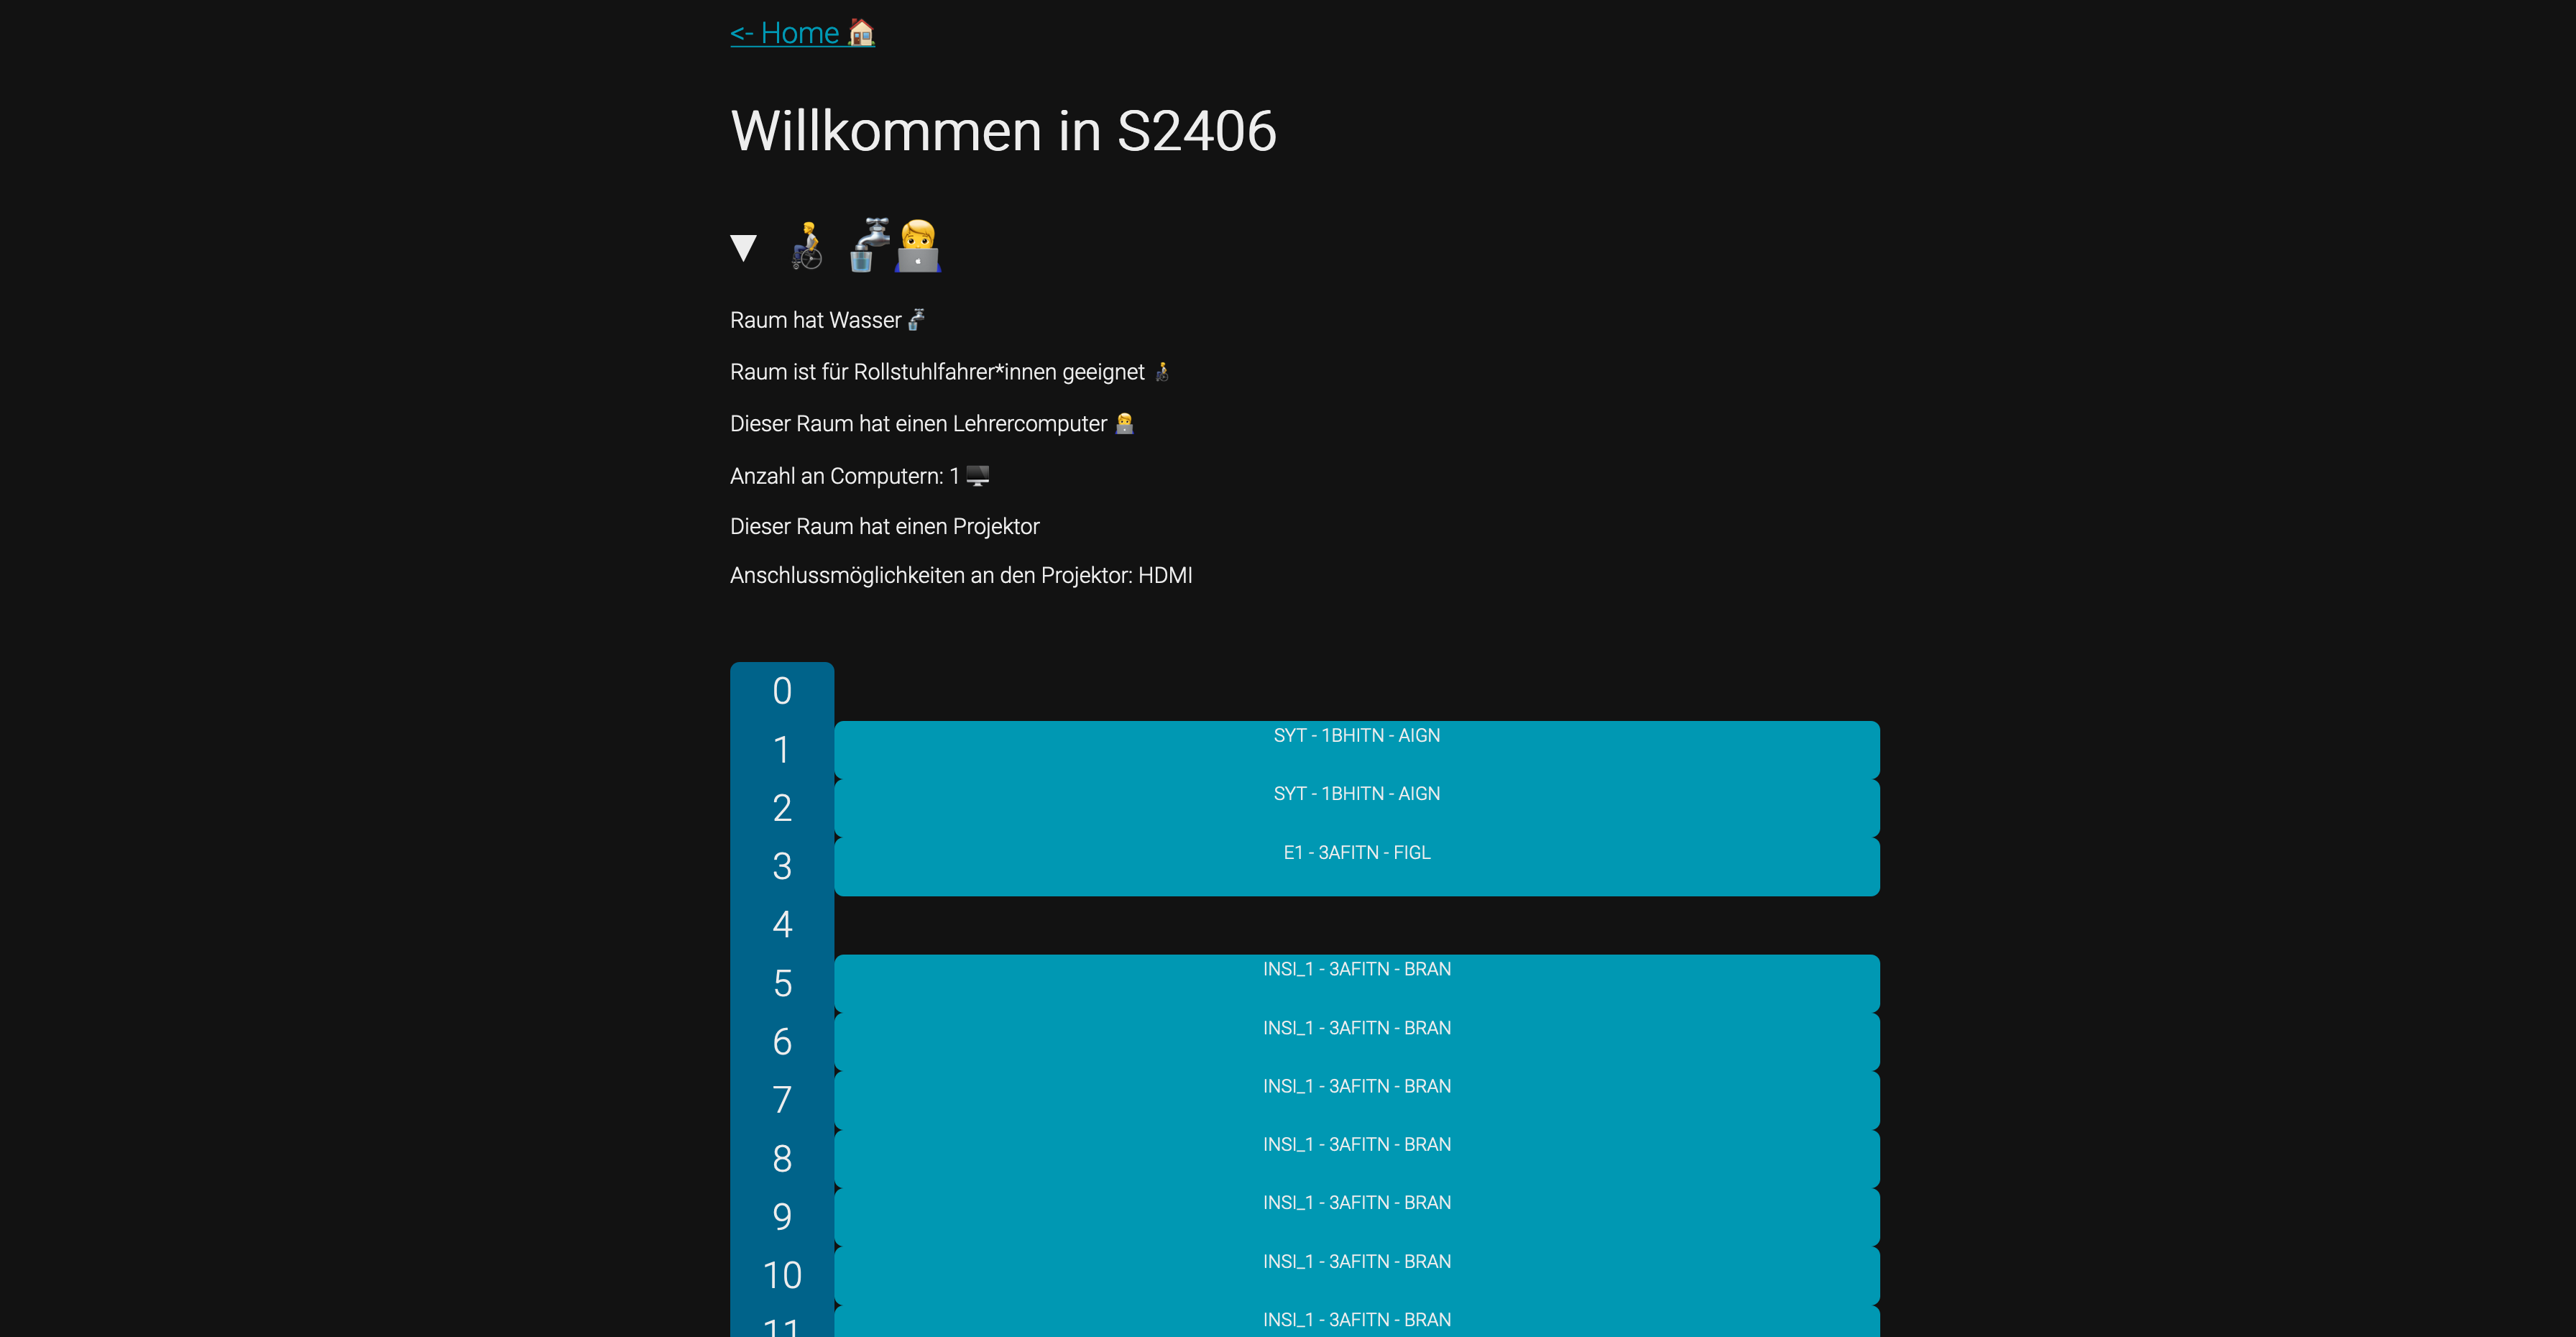
\includegraphics[width=\textwidth]{media/ResponsiveDesign/ZeliaDesktopDark.png}
        \caption{Dunkles Theme}
    \end{subfigure}
    \caption{Gegenüberstellung: helles - dunkles Theme}
    \label{fig:theme}
\end{figure}

\css[code:theme]{code/ResponsiveDesign/theme.css}{Anpassung der Farben anhand des Themes}

\clearpage
\hfour{Vergleich: Mobil und Desktop}

Da \ZELIA\ sowohl am Computer als auch am Smartphone oder Tablet genutzt werden soll, wird mithilfe der Clamp-Funktion (siehe Kapitel \ref{sec:clamp}) das Design für die verschiedenen Bildschirmgrößen angepasst (siehe Abbildung \ref{fig:info}).

\begin{figure}[H]
    \begin{subfigure}[c]{0.64\textwidth}
        \centering
        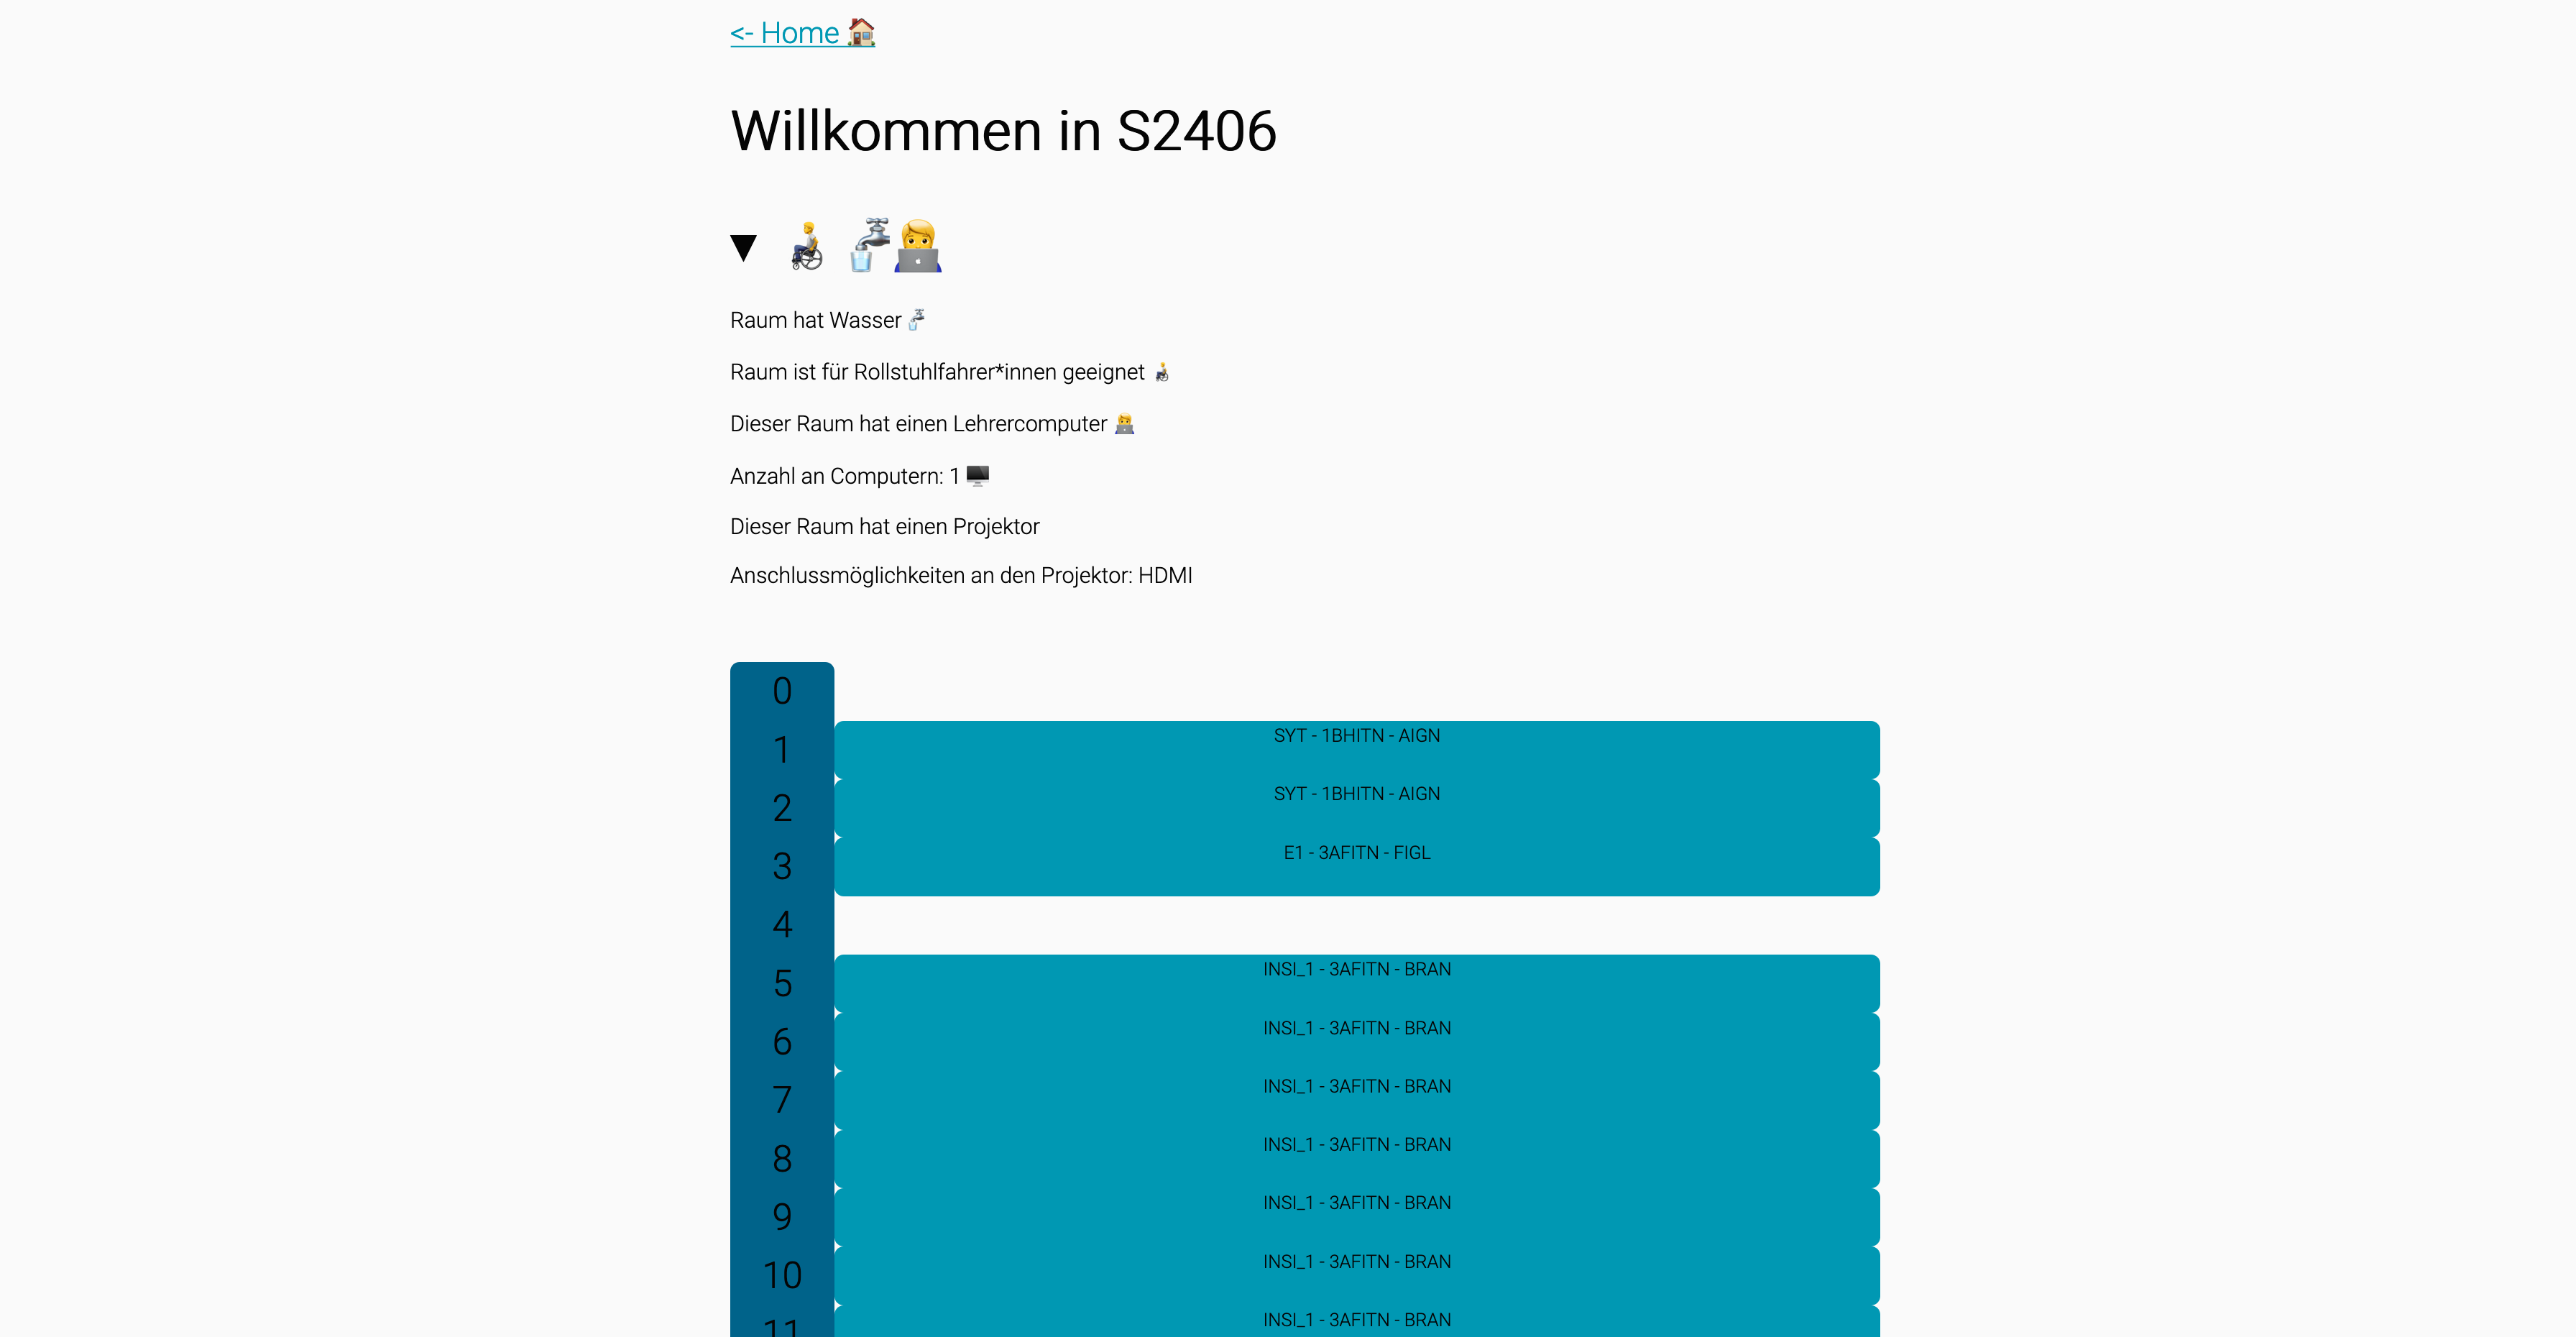
\includegraphics[width=\textwidth]{media/ResponsiveDesign/ZeliaDesktop.png}
        \caption{Rauminfo (Desktop)}
    \end{subfigure} \hfill
    \begin{subfigure}[c]{0.34\textwidth}
        \centering
        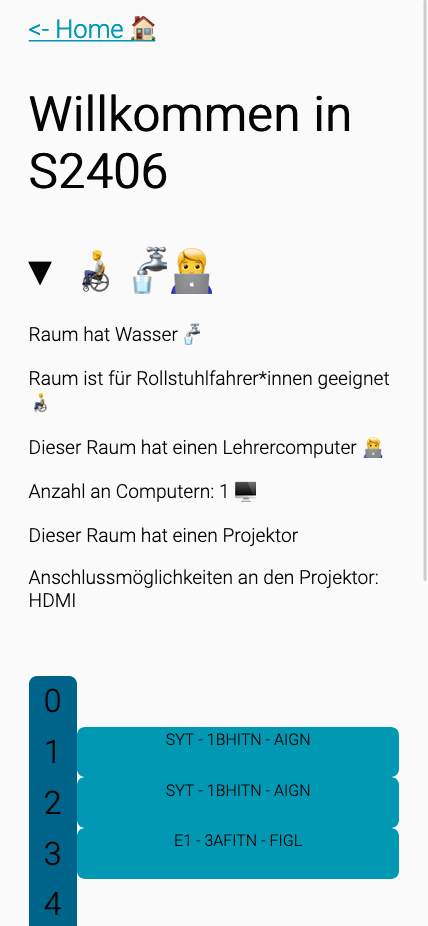
\includegraphics[width=\textwidth]{media/ResponsiveDesign/ZeliaMobile.png}
        \caption{Rauminfo (Mobil)}
    \end{subfigure}
    \caption{Vergleich von Desktop- und Mobile-Versionen der Rauminformation}
    \label{fig:info}
\end{figure}

Wenn \ZELIA\ auf einem Mobilgerät verwendet wird, dann wird der "Kamera öffnen"-Button (siehe Abbildung \ref{fig:homeMobile}) dafür angezeigt, damit die Raumnummer mittels OCR (siehe Kapitel \ref{sec:ocr}) eingelesen werden kann. Auf der Desktop-Version wird dieser Button nicht angezeigt (siehe Abbildung \ref{fig:homeDesktop}).

\begin{figure}[H]
    \begin{subfigure}[c]{0.64\textwidth}
        \centering
        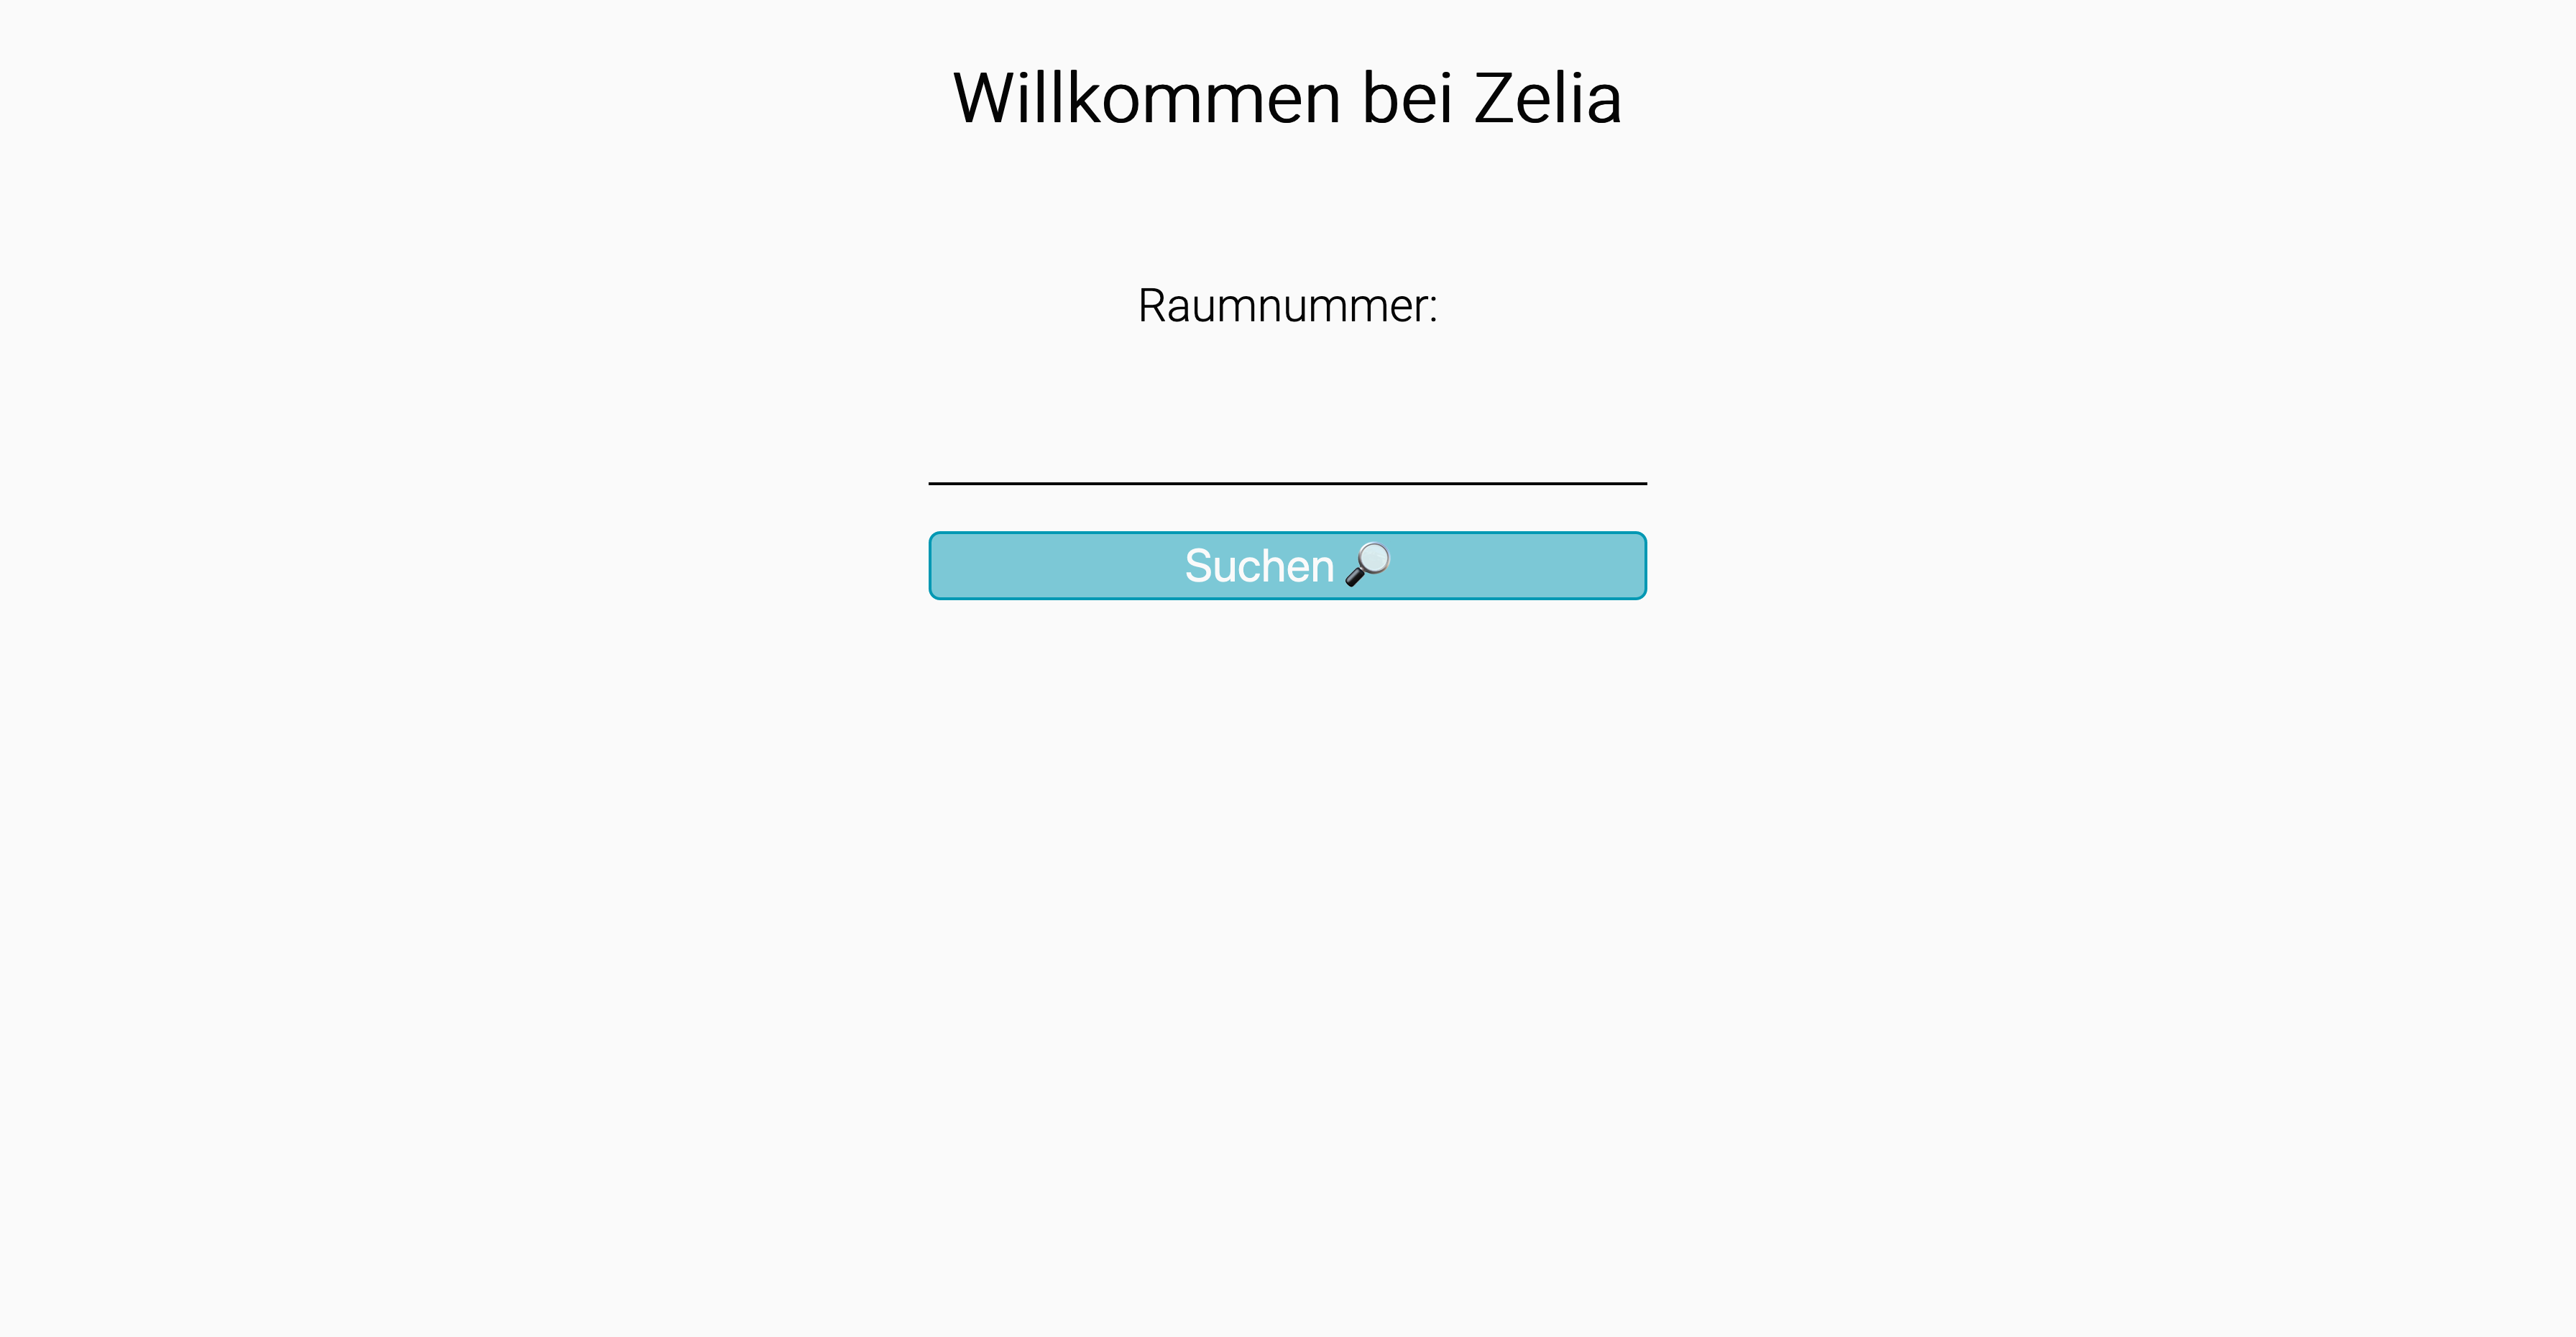
\includegraphics[width=\textwidth]{media/ResponsiveDesign/ZeliaHome.png}
        \caption{Startseite (Desktop)}
        \label{fig:homeDesktop}
    \end{subfigure} \hfill
    \begin{subfigure}[c]{0.34\textwidth}
        \centering
        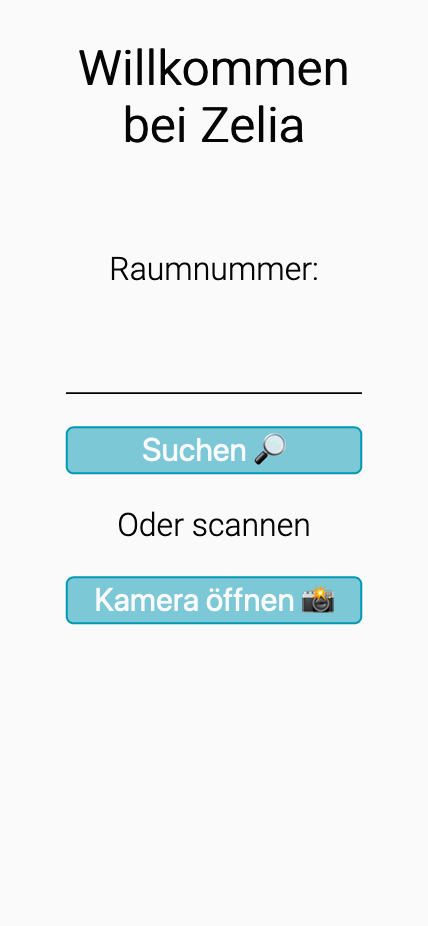
\includegraphics[width=\textwidth]{media/ResponsiveDesign/ZeliaHomeMobile.png}
        \caption{Startseite (Mobil)}
        \label{fig:homeMobile}
    \end{subfigure}
    \caption{Vergleich von Desktop- und Mobile-Version der Startseite}
    \label{fig:home}
\end{figure}